\documentclass[letterpaper,12pt]{article}

\usepackage{threeparttable}
\usepackage{geometry}
\geometry{letterpaper,tmargin=1in,bmargin=1in,lmargin=1.25in,rmargin=1.25in}
\usepackage[format=hang,font=normalsize,labelfont=bf]{caption}
\usepackage{amsmath}
\usepackage{multirow}
\usepackage{array}
\usepackage[utf8]{inputenc}
\usepackage{delarray}
\usepackage{amssymb}
\usepackage{amsthm}
\usepackage{lscape}
\usepackage{natbib}
\usepackage{setspace}
\usepackage{float,color}
\usepackage[pdftex]{graphicx}
\usepackage{pdfsync}
\usepackage{verbatim}
\usepackage{placeins}
\usepackage{geometry}
\usepackage{pdflscape}
\usepackage[procnames]{listings}
\synctex=1
\usepackage{hyperref}
\hypersetup{colorlinks, linkcolor=red, urlcolor=blue, citecolor=red, pageanchor=false}
\usepackage{bm}
\newcommand{\quotes}[1]{``#1''}



\theoremstyle{definition}
\newtheorem{theorem}{Theorem}
\newtheorem{acknowledgement}[theorem]{Acknowledgement}
\newtheorem{algorithm}[theorem]{Algorithm}
\newtheorem{axiom}[theorem]{Axiom}
\newtheorem{case}[theorem]{Case}
\newtheorem{claim}[theorem]{Claim}
\newtheorem{conclusion}[theorem]{Conclusion}
\newtheorem{condition}[theorem]{Condition}
\newtheorem{conjecture}[theorem]{Conjecture}
\newtheorem{corollary}[theorem]{Corollary}
\newtheorem{criterion}[theorem]{Criterion}
\newtheorem{definition}{Definition} % Number definitions on their own
\newtheorem{derivation}{Derivation} % Number derivations on their own
\newtheorem{example}[theorem]{Example}
\newtheorem{exercise}[theorem]{Exercise}
\newtheorem{lemma}[theorem]{Lemma}
\newtheorem{notation}[theorem]{Notation}
\newtheorem{problem}[theorem]{Problem}
\newtheorem{proposition}{Proposition} % Number propositions on their own
\newtheorem{remark}[theorem]{Remark}
\newtheorem{solution}[theorem]{Solution}
\newtheorem{summary}[theorem]{Summary}
\bibliographystyle{aer}
\newcommand\ve{\varepsilon}
\renewcommand\theenumi{\roman{enumi}}
\newcommand\norm[1]{\left\lVert#1\right\rVert}
\definecolor{codegreen}{rgb}{0,0.6,0}
\definecolor{codegray}{rgb}{0.5,0.5,0.5}
\definecolor{codepurple}{rgb}{0.0,0.0, 0.4}
\definecolor{backcolour}{rgb}{0.99,0.99,0.99}

\lstdefinestyle{mystyle}{
    backgroundcolor=\color{backcolour},
    commentstyle=\color{codegreen},
    keywordstyle=\color{magenta},
    numberstyle=\tiny\color{codegray},
    stringstyle=\color{codepurple},
    basicstyle=\scriptsize,
    breakatwhitespace=false,
    breaklines=true,
    captionpos=b,
    keepspaces=true,
    numbers=left,
    numbersep=5pt,
    showspaces=false,
    showstringspaces=false,
    showtabs=false,
    tabsize=2
}

\lstset{style=mystyle}


\begin{document}

\begin{titlepage}
\title{A Multivariate Kernel Density Estimator for the Joint Distribution of Bequest Recipients
       \thanks{
       We are grateful to the BYU Macroeconomics and Computational Laboratory and to the Open Source Policy Center at the American Enterprise Institute for research support on this project. All Python code and documentation for the computational model is available at \href{https://github.com/rickecon/OGbequests}{https://github.com/rickecon/OGbequests}. We also thank James McDonald for some helpful suggestions.}
       }
\author{
  Jason DeBacker\footnote{Middle Tennessee State University, Department of Economics and Finance, BAS N306, Murfreesboro, TN 37132, (615) 898-2528,\href{mailto:jason.debacker@mtsu.edu}{jason.debacker@mtsu.edu}.} \\[-2pt]
  \and
  Richard W. Evans\footnote{Brigham Young University, Department of Economics, 167 FOB, Provo, Utah 84602, (801) 422-8303, \href{mailto:revans@byu.edu}{revans@byu.edu}.} \\[-2pt]
  \and
  Parker Rogers\footnote{Brigham Young University, Department of Economics, 121B FOB, Provo, Utah 84602, \href{mailto:parker.rogers2@gmail.com}{parker.rogers2@gmail.com}.} \\[-2pt]}
\date{April 2016 \\
  \scriptsize{(version 16.04.a)}}
\maketitle
\vspace{-9mm}
\begin{abstract}
\small{We provide an algorithm and code for estimating a flexible joint distribution of bequest recipients in the United States by age and by net worth. Estimating this joint distribution is important in macroeconomic models with population demographics in which agents give bequest and the population is heterogeneous in terms of age and earnings ability. We use a multivariate kernel density estimator with a flexible bandwidth parameter. In addition we provide a method with accompanying code to produce the resulting discrete joint distribution over arbitrary age and lifetime income bins.

\vspace{3mm}

\noindent\textit{keywords:}\: multivariate kernel density estimation, bequests, inheritances, inter-vivos transfers, Survey of Consumer finances.

\vspace{3mm}

\noindent\textit{JEL classification:} C14, C63, D31, D91, E21}
\end{abstract}
\thispagestyle{empty}
\end{titlepage}


\begin{spacing}{1.5}

\section{Introduction}\label{SecIntro}

  In models that address wealth accumulation and inequality, careful attention must be given to transfers between agents in the form of bequests at time of death and in the form of inter-vivos transfers. A large empirical literature exists on who receives these transfers as well as who gives these transfers, although it focuses mostly on how these transfers are given and received in terms of each possible dimension heterogeneity independently. Further, the theoretical literature on wealth transfers focuses mostly on modeling the giver of the transfers and their motives.

  In this paper, we provide a contribution to both the empirical and theoretical literature on recipients of bequests. We use United States data to estimate a robust and flexible joint distribution of bequest recipients by age and net worth of recipient. This joint distribution represents a step forward in our empirical understanding of of bequest recipients. This joint distribution can also be effectively used in the theoretical literature to accurately model who receives transfers and test the persistence of wealth inequality.\footnote{The Python code for this multi-variate estimator of the joint distribution of bequest recipients is available at \href{https://github.com/rickecon/OGbequests}{https://github.com/rickecon/OGbequests}.}

  \citet{Wolff:2015} provides an expansive survey of the empirical and theoretical bequest-inheritance literature. The primary sources of U.S. data are the Survey of Consumer Finances (SCF), Panel Study of Income Dynamics (PSID), and Health and Retirement Study (HRS). The empirical portion of \citet{AltonjiEtAl:1997} focuses on the distribution of transfer recipients by income. \citet{McGarrySchoeni:1995} address a coarse distribution of transfers by age by looking at transfers to children and transfers to parents. \citet{Schoeni:1997} and \citet{WolffEtAl:2007} separately estimates the distribution of transfers received by recipient income levels and then by recipient age using data from the PSID. All four of these studies find either that transfers received decline with income or that transfers received are a U-shaped function of income. In contrast, \citet{Cox:1987}, \citet{CoxRank:1992}, \citet{Zissim:2001}, and \citet{Wolff:2015} find that transfer receipts are strongly positively correlated with income. We find this positive correlation as well. None of these studies look at the joint distribution by income and age.

  Most of the theoretical literature on bequests, inheritances, and transfers focuses on the motives of the giver.\footnote{\citet{Wolff:2015} divides these theoretical motives for giving into (i) altruism or others' wellbeing in one's utility function, (ii) exchange or giving bequests in exchange for some service, and (iii) insurance or giving bequests to others in bad times for the promise of returning the favor if bad times should arise in the future. See (i) \citet{Barro:1974}, \citet{Becker:1974}, \citet{BeckerTomes:1979}, \citet{Tomes:1981}, (ii) \citet{BernheimEtAl:1985}, \citet{Cox:1987}, and (iii) \citet{Cox:1990}, \citet{CoxJappelli:1990}, and \citet{Kochar:1997}.} Dynastic models---such as \citet{GokhaleEtAl:2001} and \citet{FarhiWerning:2010}---often assume that the wealth of one generation is divided evenly among surviving children. This does not account for proportion of bequests to grandchildren or non-family members, nor does it account for the distribution of bequests with potential disproportionality by income or ability of children or general recipients. \citet{PikettySaez:2013} do calibrate the distribution of bequest recipients and givers in their simple model....

  The current conventional wisdom among Americans is that inheritances propagate wealth inequality in the United States \citet{Wolff:2015}. In order to accurately model and predict how inheritances affect wealth inequality, we must better understand which individuals are receiving these wealth transfers. Recent literature suggests that the relationship between age and inheritance reception rates is of the form of an inverted U-shape. More specifically, the rates of inheritance reception among age groups were, 16.2\% for the youngest age group, 26.9\% for ages 55-64, and 8.3\% for ages 75+. Moreover, there is strong positive correlation between income level, and the percentage of households receiving wealth transfers \citet{Wolff:2015}.


\section{Survey of Consumer Finances Data}\label{SecSCFdata}

  The data we used was pulled from the Survey of Consumer Finances located on The Federal Reserve website. The Survey of Consumer Finances is a triennial survey conducted by The Federal Reserve that began in 1983. Each survey data set contains around 5,400 variables with over 30,000 respondents. Summary variables are included that are adjusted for inflation.\citet{FED}.

<<<<<<< HEAD
The data we used to create our MVKDE was pulled from the Survey of Consumer Finances. The Survey of Consumer Finances is a triennial survey conducted by The Federal Reserve that began in 1983. Each data set contains around 5,400 variables with over 30,000 observations. 

Another possible data source that is rich in financial information is The Panel Survey of Income Dynamics (PSID). The PSID is a cross-sectional survey conducted by The University of Michigan that began in 1968 and follows 18,000 individuals. Data can be found on employment, income, wealth, expenditures, health, marriage, childbearing, child development, philanthropy, education, and numerous other topics. \citet{UMich}

The following is a list of variables that we used from The Survey of Consumer Finances when determining our proportion matrix,
=======
  Another possible data source for our purpose is The Panel Survey of Income Dynamics (PSID). The PSID is a cross-sectional survey conducted by The University of Michigan that began in 1968 and follows 18,000 individuals. Data can be found on employment, income, wealth, expenditures, health, marriage, childbearing, child development, philanthropy, education, and numerous other topics. \citet{UMich}

  Here are the variables that we used from The Survey of Consumer Finances when determining our proportion matrix,

  X5804 - What the approximate value of the inheritances were at the time the respondent received them.
>>>>>>> upstream/master

  X5809 - The second reported value of inheritance reception.

  X5814 - The third reported value of inheritances reception.

  X5805 - The year that they received the first instance of inheritances (corresponding to X5804).

  X5810 - The year that they received the second instance of inheritances (corresponding to X5809)

  X5815 - The year that they received the third instance of inheritances (corresponding to X5814)

  X8022 - age of respondent.

  wgt - An SCF summary variable that contains the weights provided by the Federal Reserve to adjust for selection bias in the survey.

  networth - An SCF summary variable that contains the self-perceived net worth of the respondent at the time of the survey.


  Since the SCF is a triennial survey, we wanted to prevent any overlap of bequest reception between survey years. In order to do this, we used the SCF variables \quotes{X5805}, \quotes{X5810}, \quotes{X5815} as described above. These variables give the time that each instance of bequest was received, and allow us to make sure that we include only the bequests received in the current, and previous two years of the survey year. For example, the \quotes{X5804} instance of bequests was received on the year \quotes{X5805} , and if
  \[\text{\quotes{X5805}} - \text{(current~survey~year)} <3\]
  then we would include that particular instance of bequests.

  To gather the amount of bequests received, conditional upon both age and ability types (networth), we separated the bequests reported by respondents within three years of the survey by separating the bequests received by certain age and ability types into separate bins. After, we divided the amount in each age-income bin by the total amount of bequests reported within the three year interval of the survey for all respondents. This resulted in a proportion matrix, which tells us what proportion of bequests each age-income category received. Upon examining the following resulting graph of proportions over the years 2001-2013, we proceeded to apply a different variable provided by the SCF called \quotes{weights}.

  \begin{figure}[htbp]\centering \captionsetup{width=5.5in}
      \caption{\label{Weightfig}\textbf{Distribution of Inheritances Before Weights Applied}}
      \fbox{\resizebox{3.0in}{2.0in}{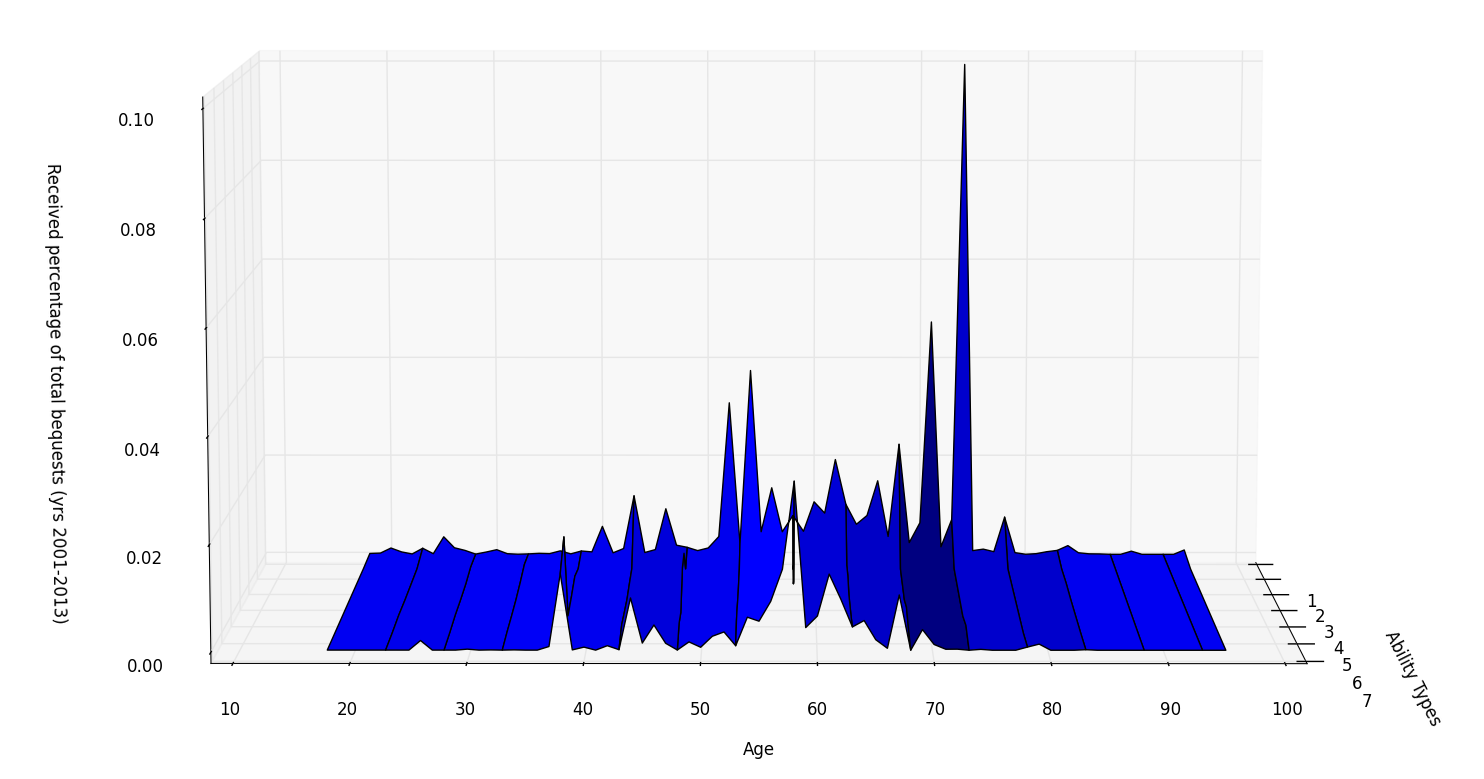
\includegraphics{withoutweights}}}
    \end{figure}
  \newpage

  In order to reduce selection bias, the SCF provides a Summary Variable called \quotes{weights}. The weights provided are meant to \quotes{compensate for unequal probabilities of selection in the original design and for unit nonresponse (failure to obtain an interview)} \citet{FEDweight}. The distribution before these weights were applied is seen in Figure \ref{Weightfig}. Notice the unnatural spike in bequest reception for individuals of age 73. We applied these weights to all our variables by multiplying the weights by each bequest value.

  Lastly, we adjusted the nominal values for bequests to account for inflation between the used survey years of 1998-2013. We used the St. Louis Federal Reserve's CPI for all urban consumers: all items \citet{StFed} . We then set 2013 as the base year and calculated the percentage inflation factors for all the years down to 1988. The inflation factors, which will be multiplied by the bequest amounts that correspond to each year, are given as follows,

  \[
  \begin{matrix}
  \hline
  1987&  1988&  1989&  1990&  1991&  1992&  1993\\

  1.51229385 & 1.492299173& 1.467973318 & 1.439144582 & 1.415496948 & 1.397721517 & 1.379834479 \\
  \hline

   1994&  1995&  1996& 1997&  1998&  1999&  2000\\

  1.363737434 & 1.345889029 & 1.326679888 & 1.310939123 & 1.300280732 & 1.284934882 & 1.260857994  \\
  \hline
   2001&2002&  2003&  2004&  2005&  2006 &2007\\

    1.240039148 & 1.227912707 & 1.210171616 & 1.189103802 & 1.161807505 & 1.134803101& 1.109966432  \\
    \hline

      2008&  2009&  2010&  2011&  2012&  2013\\

    1.076012397 & 1.078969961 & 1.063898833 & 1.034477726 & 1.014431538 & 1\\
  \hline

  \end{matrix}\]

  The final results showing the distribution of bequests received over the years 1998-2013, after applying our weights and inflation factors, are as follows,\\
  \begin{figure}[htbp]\centering \captionsetup{width=4.0in}
    \caption{\label{proportions}\textbf{Distribution of Inheritances 1998-2013}}
    \fbox{\resizebox{4.0in}{3.0in}{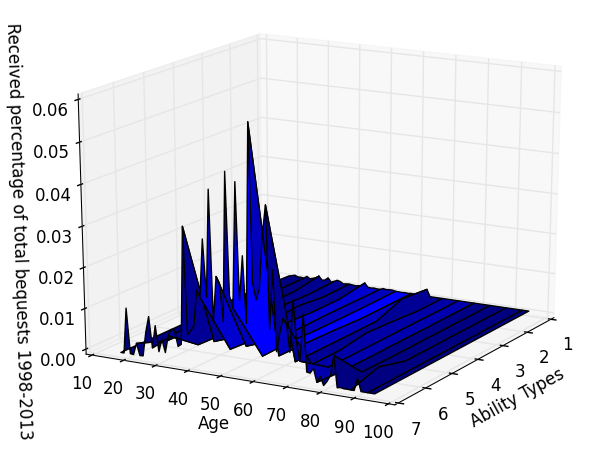
\includegraphics{result1}}}
  \end{figure}

  where the ability types one through seven are different net worth groups categorized using the following net worth amounts:

  1: Under \$15,000,

  2: \$15,000 - \$24,999,

  3: \$25,000 - \$49,999,

  4: \$50,000 - \$74,999,

  5: \$75,000 - \$99,999,

  6: \$100,000 - \$250,000,

  7: \$250,000 or more

  Notice the peak of inheritance reception at the age group 55-65 years and ability type 7. This suggests that most inheritances fall on middle-aged, wealthy individuals.

\section{Estimated Joint Distribution of Bequests}\label{SecDist}

  After gathering the data on the proportion of inheritances, we needed to fit a functional form to our data set in order to have a smooth representation of our sample and a robust way of altering both age groups and income groups according to different user inputs. For example, if the user wanted only four ability-type cohorts and twenty age cohorts, then we need a way to create new proportion bins according to these specified conditions. If we were to use only our sparse non-linear data set, it would be difficult to compose the desired proportions for each age-ability category. However, a functional form allows us to impose any conditions on the bequest distribution that the user desires. This is why we chose to fit a Multivariate Kernel Density Estimator to our data set.


  \subsection{Multivariate Kernel Density Estimator (MVKDE)}\label{SecDistMVKDE}

    Kernel Density Estimation is a non-parametric way to approximate a density function when the parametric form of the sampling density is unknown. This proved to be useful in our approximation of the underlying density function of our data in Figure \ref{proportions}. We used a Multivariate Kernel Density Estimator to estimate the sample density as there were no clear parametric density forms that matched our data set. We put forward both the univariate and the multivariate Kernel Density Estimators, and display our Python code used to execute this estimation.

    The Univariate Kernel Density Estimator is defined as follows:

    \[\hat{f}(x) = \frac{1}{nh} \sum_{i=1}^n K\Big(\frac{x-x_i}{h}\Big)= \frac{1}{n}\sum_{i=1}^n K_h (x - x_i) \quad \]

    where $K_h(x) =  K(x/h)/x$ is the kernel function of choice, $h$ is the bandwidth, and $n$ is the number of sample points \citet{Scott:2015}. Much like the histogram, a Kernel Density Estimator, creates functional values that correspond to a chosen kernel function at each sample point. Moreover, upon summing up each kernel function corresponding to its respective sample point, this sum of kernels is evenly scaled by dividing the functional values by the total number of sample points and the bandwidth selection.

    The multivariate case of kernel estimation is given by the following,
    \[\hat{f}_\mathbf{H}(\mathbf{x})= \frac1n \sum_{i=1}^n K_\mathbf{H} (\mathbf{x} - \mathbf{x}_i)\]

    In our case, we used a Gaussian Kernel , which yields the following equation for this general Multivariate Kernel Density Estimator for $\mathbf{x} \in \mathbb{R}^d$

    \[\hat{f}(\mathbf{x}) = \frac{1}{n2\pi ^{d/2} |\Sigma|^{1/2}} \sum_{i=1}^n \text{exp}\big[-\frac{1}{2}(x-x_i)^T\Sigma ^{-1}(x-x_i)\big]\]
    \citet{Scott:2005}

    In order to implement our Multivariate Kernel Density Estimator we used the following python code,\\

    \begin{lstlisting}[language=Python, caption=MVKDE.py]
      import numpy as np
      from matplotlib import pyplot as plt
      from mpl_toolkits.mplot3d import Axes3D
      from scipy import stats
      from scipy.stats import norm
      from scipy.stats import kde

      def MVKDE(s, e, filename, plot = False):
        '''
        Generates a Multivariate Kernel Density Estimator and returns a matrix
        representing a probability distribution according to given age categories,
        and ability type categories.

        Inputs:
            s             = scalar, the number of age groups in the model.

            e             = scalar, the number of ability type groups in the model.

            filename      = string, the file name of the .txt document that contains
                            the original proportion matrix created by SCFExtract.py.

            plot          = boolean, whether or not you want a plot of the probability
                          distribution generated by your given age and ability type
                          groups.

        Functions called:
          kde.gaussian_kde      = scipy function that generates a Kernel
                                  Density Estimator from given data

        Objects in function:
            proportion_matrix     = [78, 7], array containing the proportion (0 < x < 1) of
                                    the total bequests that each age-income category receives.
                                    Derived in SCFExtract.py

          age_probs             = [78,], array containing the frequency, or how many times,
                                    that random drawn numbers fell into the 78 different age bins

          income_probs          = [7,], array containing the frequency, or how many times,
                                    that random drawn numbers fell into the 7 different ability
                                    type bins

          age_frequency         = [70000,], array containing repeated age values for each
                                    age number at the frequency given by the age_probs vector

          xmesh                 = complex number, the number of age values that will be
                                    evaluated in the Kernel Density Estimator.

          freq_mat              = [70000, 2], array containing age_frequency and
                                    income_frequency stacked

          density               = object, class given by scipy.stats.gaussian_kde.
                                    The Multivariate Kernel Density Estimator for the given data set.

          age_min, age_max      = scalars, the minimum and maximum age values and minimum
            income_min, income_max  and maximum income values


          agei            = [s, e], array containing the age values to be evaluated in
                                    the Kernel Estimator (ranging from 18-90)

          incomei         = [s, e], array containing the income values to be evaluated
                                    in the Kernel Estimator (ranging from 1-7)

          coords                = [2, s*e], array containing the raveled values of agei
                                    and incomei stacked

          estimator             = [s, e], array containing the new proportion values for
                                    s age groups and e ability type groups that are evaluated
                                    using the Multivariate Kernel Density Estimator

          estimator_scaled       = [s, e], array containing the new proportion values for
                                    s age groups and e ability type groups that are evaluated using
                                    the Multivariate Kernel Density Estimator, but scaled so that
                                    the sum of the array is equal to one.

          Returns: estimator_scaled
          '''

        proportion_matrix = np.loadtxt(filename, delimiter = ',')
        proportion_matrix_income = np.sum(proportion_matrix, axis = 0)
        proportion_matrix_age = np.sum(proportion_matrix, axis = 1)
        age_probs = np.random.multinomial(70000,proportion_matrix_age)
        income_probs = np.random.multinomial(70000, proportion_matrix_income)
        age_frequency = np.array([])
        income_frequency = np.array([])
        age_mesh = complex(str(s)+'j')
        income_mesh = complex(str(e)+'j')

        j = 18
        '''creating a distribution of age values'''
        for i in age_probs:
          listit = np.ones(i)
          listit *= j
          age_frequency = np.append(age_frequency, listit)
          j+=1

        k = 1
        '''creating a distribution of ability type values'''
        for i in income_probs:
          listit2 = np.ones(i)
          listit2 *= k
          income_frequency = np.append(income_frequency, listit2)
          k+=1

        freq_mat = np.vstack((age_frequency, income_frequency)).T
        density = kde.gaussian_kde(freq_mat.T, bw_method=0.3)
        age_min, income_min = freq_mat.min(axis=0)
        age_max, income_max = freq_mat.max(axis=0)
        agei, incomei = np.mgrid[age_min:age_max:age_mesh, income_min:income_max:income_mesh]
        coords = np.vstack([item.ravel() for item in [agei, incomei]])
        estimator = density(coords).reshape(agei.shape)
        estimator_scaled = estimator/float(np.sum(estimator))
        if plot == True:
          fig = plt.figure()
          ax = fig.gca(projection='3d')
          ax.plot_surface(agei,incomei, estimator_scaled, rstride=5)
          ax.set_xlabel("Age")
          ax.set_ylabel("Ability Types")
          ax.set_zlabel("Received percentage of total bequest")
          plt.show()
        return estimator_scaled

      newproportion =  MVKDE(80,7,'fileout.txt', True)
    \end{lstlisting}

    We used the kernel function from the imported scipy module for our estimation. This kernel function works much like a histogram, therefore we changed the nature of our data from a matrix of proportions to vectors filled with the frequencies that different age and ability type groups occurred. This transformation occurs on lines 80-103.

    Using the multinomial function from numpy, we loaded the function with our proportion vectors for age and ability type. We obtained these vectors by summing up our proportion matrix over both the age and then the ability type axes. This resulted in two vectors that summed to one, which provide the proportions that each age group and ability type group received. The multinomial function then uses those proportions as probabilities and takes random draws according to those given proportions. We specified the function to take 70,000 random draws with the given probabilities that correspond to the age and ability proportions. For our age probability vector, this creates a new vector where each index corresponds to an age group in ascending order (18-95), where each index contains the number of times that a random draw resulted in that particular age. For our ability probability vector, multinomial creates a similar vector in ascending order (1-7), with the number of draws that fell into into each ability type group/index.

    After creating these vectors we created two new vectors that transform the data set from proportions to age numbers and ability type numbers. The frequency that each age and ability type number occurs is determined by how many times the random draw from our multinomial function resulted in each age and ability type respectively. For example, if our \quotes{age\_probs} vector contains 1,876 at index 0, then this means that age 18 was drawn 1,876 times. This means that we would put 1,876 instances of \quotes{18} in our new vector called \quotes{age\_frequency}. This is done similarly with our \quotes{income\_probs} and \quotes{income\_frequency} vectors.

    These new vectors now correspond to the required data format for scipy's kernel function. We then create the appropriate mesh grid to be entered into the \quotes{density} estimator function. Finally we scale the estimate to sum to one, and graph the resulting estimator.


  \subsection{Distribution of bequests}\label{SecDistEst}

    Our results for a Multivariate Kernel Density Estimator are illustrated in the following graph,\\

    \begin{figure}[htbp]\centering \captionsetup{width=6.0in}
      \caption{\label{MVKDE}\textbf{MVKDE of Distribution of Inheritances 1998-2013}}
      \fbox{\resizebox{4.0in}{3.0in}{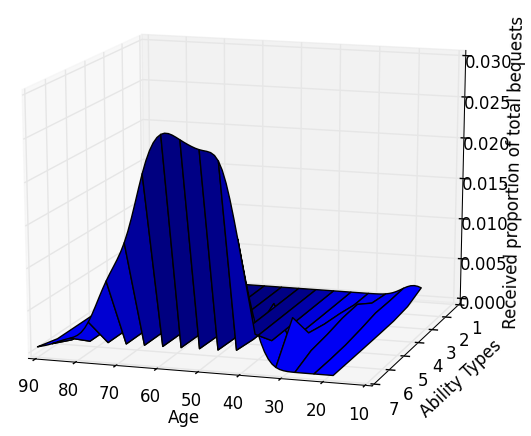
\includegraphics{KernelEstimator}}}
    \end{figure}

    Note that the peak of bequest reception still lies in the age group 55-65 years and ability type 7 like Figure \ref{proportions}. Our estimated distribution is ultimately defined by a matrix of proportions whose dimensions are determined by the user. In this particular case, we specified 78 age groups (ages 18-95) and 7 ability type groups. Any desired amount of age groups and ability type groups can be given, and the resulting matrix will match these amounts. This flexibility allows our distribution to change and alter according to the different specifications in macroeconomic models.

    Also, a noteworthy characteristic of the MVKDE is the use of a bandwidth parameter. This parameter allows for the graph to be more or less smooth. Smoothness corresponds to higher values of the \quotes{bw\_method} in the \quotes{kde.gaussian\_kde} function, and represents a distribution that is less determined by the data. The lower the bandwidth selection, the rougher the graph is and the more jagged the distribution; however, the lower bandwidths more accurately portray the behavior of the sample set.


\section{Conclusion}\label{SecConclusion}

  Our estimation of a bequest distribution allows for a data-driven allocation of inheritances among different age and ability type groups. This allows for more heterogeneity among agents within macroeconomic models, and can ultimately lead to more accurate results. Previous methods of bequest allocation in dynamic macroeconomic models are most assuredly not true. The assumption that inheritances are distributed equally among different income groups, or that they are distributed only to individuals who belong to the same income group as those giving the inheritances, is not true according to our sample. By using a more accurate distribution of inheritances we can better predict the effects that inheritance taxes have on the distribution of wealth.

  By modeling our distribution using a MVKDE, we are able to have flexible age and ability categories. If a macroeconomic model is defined by 3-period lived agents, then one can input the need for three distinct age categories, and the resulting estimated proportion matrix will be returned with three rows representing the three age groups. Similarly, if a model defines five ability type groups in the economy, our estimator can return a new matrix of proportions with five columns of ability types. This flexibility will allow this estimator to be used in a wide variety of macroeconomic models.

  Even though we were able to find data in The Survey of Consumer Finances regarding individuals who receive bequests by both age and income, we were unable to find data that links these individuals with those who are giving bequests. It would be useful to know which individuals, by age and income categories, are giving bequests so that we can also accurately model this component of bequest distribution.



\clearpage


\end{spacing}


\newpage
\bibliography{KDbequests}


% \newpage
% \renewcommand{\theequation}{A.\arabic{section}.\arabic{equation}}
%                                                  % redefine the command that creates the section number
% \renewcommand{\thesection}{A-\arabic{section}}   % redefine the command that creates the equation number
% \setcounter{equation}{0}                         % reset counter
% \setcounter{section}{0}                          % reset section number
% \section*{APPENDIX}                              % use *-form to suppress numbering

% \section{First Appendix Section Title}\label{AppTitle1}

%   Put first Appendix section content here.


% \newpage
% \section{Second Appendix Section Title}\label{AppTitle2}

%   \setcounter{equation}{0}

%   Put second Appendix section content here.



\end{document}
